\documentclass{standalone}
\usepackage{pgfplots}
\pgfplotsset{width=7cm,compat=1.8}

\usepackage{unicode-math}
\usepackage{siunitx}


\begin{document}

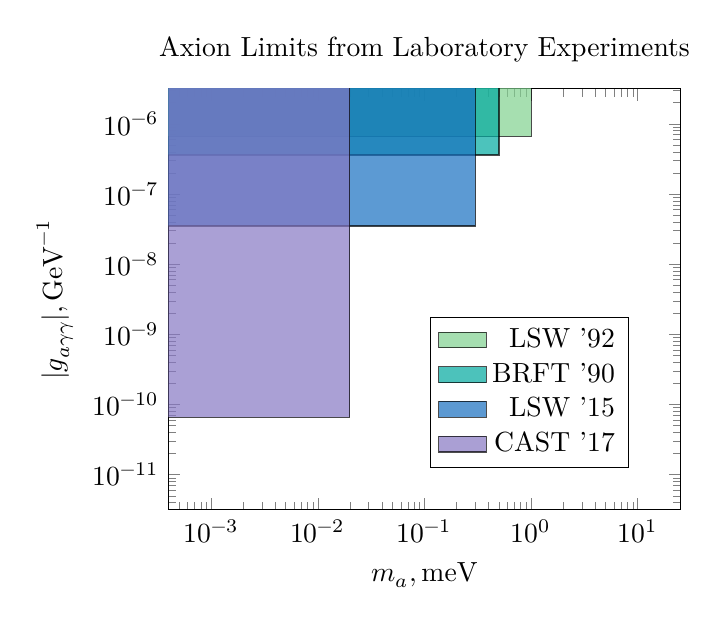
\begin{tikzpicture} 
	\begin{loglogaxis}[
		scale=1.2,
		enlargelimits=0.1,
		ymin=1e-11, ymax=1e-6,
		xmin=1e-3, xmax=1e1,
		xlabel={$m_a, \si{\milli\eV}$},
		ylabel={$|g_{aγγ}|, \si{\per\giga\eV}$},
	    legend style={
	    	at={(0.9,0.1)},
	    	anchor=south east,
	    	legend cell align=right,
	    },
	    title={Axion Limits from Laboratory Experiments},
	    every axis plot/.append style={
	    	area legend,
	    	opacity=0.7,
    	},
	]
	% \addplot [thick,color=blue, fill=blue, fill opacity=0.1]
	% coordinates {
	% 		(1, 1)
	% 	(1, 6.7e-7)
	% 		(0.5, 6.7e-7)
	% 	(0.5, 3.6e-7)
	% 		(0.3, 3.6e-7)
	% 	(0.3, 3.5e-8)
	% 		(0.02, 3.5e-8)
	% 	(0.02, 6.6e-11)
	% 		(1e-4, 6.6e-11)
	% 		(1e-4, 1)
	% };
	% \addplot[mark=x, only marks, color=blue] coordinates {
	% 	(1, 6.7e-7)
	% 	(0.5, 3.6e-7)
	% 	(0.3, 3.5e-8)
	% 	(0.02, 6.6e-11)
	% };

	\addplot [fill=cyan!50!yellow] coordinates {
			(1e-4, 1)
			(1, 1)
		(1, 6.7e-7)
			(1e-5, 6.7e-7)
	};
	\addplot [fill=cyan!50!green] coordinates {
			(1e-4, 1)
			(0.5, 1)
		(0.5, 3.6e-7)
			(1e-5, 3.6e-7)
	};
	\addplot [fill=cyan!50!blue] coordinates {
			(1e-4, 1)
			(0.3, 1)
		(0.3, 3.5e-8)
			(1e-5, 3.5e-8)
	};
	\addplot [fill=cyan!50!magenta] coordinates {
			(1e-4, 1)
			(0.02, 1)
		(0.02, 6.6e-11)
			(1e-5, 6.6e-11)
	};

	% \addplot [fill=blue!50!red, opacity=0.7, area legend] coordinates {
	% 	(0.7, 1e-12)
	% 	(0.7, 1e-5)
	% 	(300e3, 1e-5)
	% 	(300e3, 1e-12)
	% };

	\legend{
		LSW '92,
		BRFT '90,
		LSW '15,
		CAST '17,
		% Cosmo
	}
	\end{loglogaxis}
\end{tikzpicture}  	

\end{document}
